\graphicspath{{figures/tornado/}}
\chapter{龙卷风风场及其数值模拟}\label{chapter:tornado}

% \section{计算流体动力学基本理论}
计算流体动力学(Computational Fluid Dynamics, CFD)是通过数值方法在计算机中对流
体力学的控制方程(质量守恒方程、动量守恒方程、能量守恒方程)进行求解,从而可预测
流场的流动。
CFD技术的基本思路可归纳为:把时间域及空间域上连续的物理量(如压力场、速度场),
用一系列的有限离散点上变量值得集合来代替,通过一定的原则和方式建立关于离散点上场
变量之间关系的代数方程组,然后求解此代数方程组获得场变量的近似值。

CFD克服了传统的理论分析和试验研究的缺点,不受物理模型和试验模型限制,经济、高效、
灵活,能够给出较为完整的数据和图像。
尤其对特殊情况如试验无法模拟的时候,CFD将会发挥出独特的优势。

\subsection{控制方程}

流体的流动要受物理守恒定律的支配,包括质量守恒定律、动量守恒定律和能量守恒定律。
控制方程是这些守恒定律的数学描述。

\subsubsection{质量守恒方程}
质量守恒定律可表述为:单位时间内流体微元体中质量的增加量,等于同一时间间隔内流入
该微元体的净质量。
根据这一定律,可得到流体的质量守恒定律(连续方程):
\begin{equation}
  \label{eq:continuity}
  \frac{\partial \rho}{\partial t} + \mathrm{div} (\rho \bm{u}) = 0
\end{equation}
式中:$ \rho $为空气密度,$ t $是时间,$ \bm{u} $为空气的速度矢量,$ u $、$ v $、
$ w $是速度矢量$ \bm{u} $在$ x $、$ y $、$ z $三个方向上的分量,$ \mathrm{div}
(\bm{a}) = \frac{\partial a_x }{\partial x } + \frac{\partial a_y }{\partial y }
+ \frac{\partial a_z  }{\partial z } $为矢量$ \bm{a} $的散度。

\subsubsection{动量守恒方程}
动量守恒定律可以表述为:流体微元体中流体动量对时间的变化率等于外界作用在该微元体
上的各种力之和,该定律实际上是牛顿第二定律。
据此,可推导出$ x $、$ y $、$ z $ 三个方向的动量守恒方程:
\begin{equation}
  \label{eq:momentum}
  \begin{cases}
    \rho \frac{\mathrm{d} u }{\mathrm{t}} = -\frac{\partial p}{\partial x} +
    \frac{\partial \tau_{xx}}{\partial x} + \frac{\partial \tau_{yx}}{\partial y} +
    \frac{\partial \tau_{zx}}{\partial z} + F_x \\
    \rho \frac{\mathrm{d} v }{\mathrm{t}} = -\frac{\partial p}{\partial y} +
    \frac{\partial \tau_{xy}}{\partial y} + \frac{\partial \tau_{yy}}{\partial y} +
    \frac{\partial \tau_{zy}}{\partial z} + F_y \\
    \rho \frac{\mathrm{d} w }{\mathrm{t}} = -\frac{\partial p}{\partial z} +
    \frac{\partial \tau_{xz}}{\partial x} + \frac{\partial \tau_{yz}}{\partial y} +
    \frac{\partial \tau_{zz}}{\partial z} + F_z \\
  \end{cases}
\end{equation}
式中:$p$为流体微元体上的压力;$\tau_{xx}$、$\tau_{xy}$、$\tau_{xz}$分别为因粘性
作用而产生的作用在微元体表面上粘性应力的分量;$F_x$、$F_y$和$F_z$是微元体上的体
力分量,当微元体受到的体力只有重力,且$z$轴的方向竖直向上时,体力可以写成:
$F_x=0$,$F_y=0$,$F_z=-\rho g$。

下面对流体的粘性应力进行分析。当相邻两层流体发生相对滑移(即剪切变形)时,在与变
形相反方向上会产生粘性应力(切向应力),来阻止变形的发生。
流体这种抵抗变形的性质,称为粘性。
结构风工程中的研究对象主要为近地层的空气,一般可看成是牛顿粘性流体。
对于牛顿粘性流体,流体的粘性应力与其变形率成比例,各分量可写成如下形式:
\begin{equation}
  \label{eq:newton}
  \begin{cases}
    \tau_{xx}=2\mu \frac{\partial u}{\partial x} + \lambda \mathrm{div} \bm{u} \\
    \tau_{yy}=2\mu \frac{\partial v}{\partial y} + \lambda \mathrm{div} \bm{v} \\
    \tau_{zz}=2\mu \frac{\partial w}{\partial z} + \lambda \mathrm{div} \bm{w} \\
    \tau_{xy}=\tau_{yx}=\mu \left( \frac{\partial u}{\partial y} +
      \frac{\partial v}{\partial x} \right) \\
    \tau_{xz}=\tau_{zx}=\mu \left( \frac{\partial u}{\partial z} +
      \frac{\partial w}{\partial x} \right) \\
    \tau_{yz}=\tau_{zy}=\mu \left( \frac{\partial v}{\partial z} +
      \frac{\partial w}{\partial y} \right)
  \end{cases}
\end{equation}
式中,$\mu$是动力粘度,$\lambda$为第二粘度,一般可取$\lambda=-\frac{2}{3}\mu$。
将式\eqref{eq:newton}代入式\eqref{eq:momentum}中,可得到牛顿流体的动量方程,也就
是比较常见的Navier-Stokes方程:
\begin{equation}
  \label{eq:ns}
  \begin{cases}
    \frac{\partial (\rho u)}{\partial t} + \mathrm{div}(\rho u \bm{u}) =
    \mu  \bm{\mathrm{grad} }(u) - \frac{\partial p}{\partial x} + S_u \\
    \frac{\partial (\rho v)}{\partial t} + \mathrm{div}(\rho v \bm{u}) =
    \mu \bm{\mathrm{ grad} }(v) - \frac{\partial p}{\partial y} + S_v \\
    \frac{\partial (\rho w)}{\partial t} + \mathrm{div}(\rho w \bm{u}) =
    \mu \bm{\mathrm{ grad} }(w) - \frac{\partial p}{\partial x} + S_w
  \end{cases}
\end{equation}
式中,$\bm{\mathrm{grad}}() = \frac{\partial ()}{\partial x} \bm{i} + \frac{\partial
  ()}{\partial y} \bm{j} + \frac{\partial ()}{\partial z} \bm{k}$为变量的梯度;
$S_u$、$S_v$、$S_w$代表着动量守恒方程的广义源项,其中$S_u=F_x+s_x$,
$S_v=F_y+s_y$,$S_w=F_z+s_z$,一般情况下,$s_x$、$s_y$、$s_z$是小量,此处不再列
出,对于粘性为常数的不可压缩流体,可取$s_x=s_y=s_z=0$。

\subsubsection{能量守恒方程}
能量守恒定律是包含有热交换的流动系统必须满足的基本规律,能量守恒定律可表述为:流
体微元体中能量的增加率等于进入微元体的净热流量加上体力与面力对微元体所做的功。
该定律实际上是热力学第一定律。
\begin{equation}
  \label{eq:energy}
  \frac{\partial \rho T}{\partial t} + \mathrm{div} (\rho \bm{u} T) =
  \mathrm{div} \left( \frac{K}{c_P} \bm{\mathrm{grad}} T \right) + S_T
\end{equation}
式中:$T$是流体的温度,$K$是流体的传热系数,$c_p$是比热容,$S_T$是流体的内热源及
由于粘性作用流体机械能转换为热能的部分,有时简称$S_T$为粘性耗散项。

综合方程\eqref{eq:continuity}、\eqref{eq:ns}、\eqref{eq:energy}等五个方程,共有
$u$、$v$、$w$、$p$、$T$和$\rho$六个未知量,还需要补充一个流体的状态方程,方程组
才能封闭:
\begin{equation}
  \label{eq:state}
  p = p(\rho, T)
\end{equation}

由于近地边界层中的风速一般小于$0.3$倍的声速,因此可近似将近地层中的空气看成不可
压缩的气体,即空气的密度是一个常量,不是空间或空间的函数。
对于不可压缩流动,若热量交换很少以致可以忽略,可不考虑能量守恒方程。
这样,只要联立求解质量守恒方程\eqref{eq:continuity}和动量守恒方程\eqref{eq:ns}即
可。
四个未知数$u$、$v$、$w$、$p$,四个方程,方程组封闭。

\subsection{湍流模型}

雷诺在1883年通过圆管试验揭示了粘性流体存在着两种不同的流动形态:层流和湍流。
当雷诺数小于某一临界值,相邻的流动层彼此能有序地流动互不干扰,这种流动称为层流;
当雷诺数大于该临界值时,流动呈现出无序的混乱状态,它的流动特征量(如速度、压强等)
随机变化,这种流动状态称为湍流。
大气边界层中的空气流动状态一般属于湍流。
湍流流动的主要特征是运动过程中流体质点发生不断互相混掺的现象,速度和压力等物理量
是在空间和时间上均具有随机性质的脉动值。

上文所述的质量守恒方程\eqref{eq:continuity}和Navier-Stokes动量方程\eqref{eq:ns},对于
层流和湍流都是适用的。
但对湍流流动,直接求解三维瞬态控制方程,对计算机的内存和速度要求很高,目前在工程
实际中不可能实现。
对于湍流流动,工程中采用的比较多的是大涡模拟(LES)和雷诺平均(RANS)两种方法。
大涡模拟(LES)的基本思路为:用瞬态的Navier-Stokes方程直接模拟湍流中的大尺度涡,
并不直接模拟小尺度涡,通过近似的模型来考虑小涡对大涡的影响。
而雷诺平均(RANS)方法是对瞬态控制方程做时间平均处理,同时补充反映湍流特性的其他
方程如湍流动能方程和湍流耗散率方程等。

将三维瞬态控制方程中的各变量写成其平均值与脉动值相加的形式,如式
\eqref{eq:rans-v}和式\eqref{eq:rans-p}所示。
$\bm{u}^{*}$表示流体的速度矢量瞬时值,$\bm{u}$表示流体的速度矢量平均值,
$\bm{u}^{'}$表示流体的速度矢量脉动值。其他变量以此类推。
将其代入瞬态连续方程\eqref{eq:continuity}和Navier-Stokes方程\eqref{eq:ns}中,并
在方程两侧对时间取平均,可以得到湍流时均流动的控制方程。
\begin{equation}
  \label{eq:rans-v}
  \bm{u}^{*} = \bm{u} + \bm{u}^{'}
\end{equation}
\begin{equation}
  \label{eq:rans-p}
  p^{*} = p + p^{'}
\end{equation}

时均量表示的连续方程(质量守恒方程):
\begin{equation}
  \label{eq:continuity2}
  \frac{\partial \rho}{\partial t} + \mathrm{div} (\rho \bm{u}) = 0
\end{equation}

时均量表示的动量方程(Navier-Stokes方程):
\begin{equation}
  \label{eq:ns2}
  \begin{cases}
    \frac{\partial (\rho u)}{\partial t} + \mathrm{div}(\rho u \bm{u}) =
    \mathrm{\mu \bm{grad} u} - \frac{\partial p}{\partial x} +
    \rho \left( -\frac{\partial \left( \rho \overline{u^{'2}} \right)}{\partial x}
    -\frac{\partial \left( \rho \overline{u^{'}v^{'}} \right)}{\partial y}
    -\frac{\partial \left( \rho \overline{u^{'}w^{'}} \right)}{\partial z}\right)
    + S_u \\
    \frac{\partial (\rho v)}{\partial t} + \mathrm{div}(\rho v \bm{u}) =
    \mathrm{\mu \bm{grad} v} - \frac{\partial p}{\partial y} +
     \rho \left( -\frac{\partial \left( \rho \overline{u^{'}v^{'}} \right)}{\partial x}
    -\frac{\partial \left( \rho \overline{v^{'2}} \right)}{\partial y}
    -\frac{\partial \left( \rho \overline{v^{'}w^{'}} \right)}{\partial z}\right)
    + S_v \\
    \frac{\partial (\rho w)}{\partial t} + \mathrm{div}(\rho w \bm{u}) =
    \mathrm{\mu \bm{grad} w} - \frac{\partial p}{\partial x}
     \rho \left( -\frac{\partial \left( \rho \overline{u^{'}w^{'}} \right)}{\partial x}
    -\frac{\partial \left( \rho \overline{v^{'}w^{'}} \right)}{\partial y}
    -\frac{\partial \left( \rho \overline{w^{'2}} \right)}{\partial z}\right)
    + S_w
  \end{cases}
\end{equation}

从公式\eqref{eq:ns2}中可看出,时均流动的动量方程又出现了新的未知项
$\rho \overline{u_i^{'} u_j^{'}}$。
人们定义该未知项为雷诺应力项,用$\tau_{ij}$表示:
\begin{equation}
  \label{eq:reynolds}
  \tau_{ij} = -\rho \overline{u_i^{'} u_j^{'}}
\end{equation}

雷诺应力由湍流脉动值所引起的应力张量,为未知量。
必须引入新的湍流模型,才能使得时均化的连续方程\eqref{eq:continuity2}和时均化的动
量守恒方程\eqref{eq:ns2}构成的方程组封闭求解。
一般通过湍流模型将湍流脉动值与时均值联系起来。
由于没有特定的物理规律可以用来指导建立湍流模型,因此目前的湍流模型只能以大量实验
观测结果作为基础。
雷诺应力的求解是各湍流闭合模型的核心问题。
根据对雷诺应力做出的假定或处理方法,可以将湍流模型分为两类:雷诺应力模型和涡粘模
型。
其中雷诺应力模型方法是直接构建雷诺应力的方程,然后联立求解质量守恒方程和动量守恒
方程和新构建的雷诺应力方程。
涡粘模型方法中,并不直接处理雷诺应力项,而是引入湍动粘度或涡粘系数,把湍流应力表
示成湍动粘度的函数。

涡粘模型方法中的湍动粘度来源于Boussinesq提出的涡粘假定,该假定建立了雷诺应力相对
于平均速度梯度的关系,即:
\begin{equation}
  \label{eq:bou}
  -\overline{u_i^{'} u_j^{'}} = \upsilon_t \left( \frac{\partial u_i}{\partial x_j} +
    \frac{\partial u_j}{\partial x_i}\right)
  - \frac{2}{3} \delta_{ij} k
\end{equation}
式中,$\upsilon_t$是湍动涡粘性系数,取决于流动状态;
$u_i$是流体的时均速度;$\delta_{ij}$为Kronecker delta符号(当$i=j$时,
$\delta_{ij}=1$;当$i \neq j$时,$\delta_{ij}=0$);
$k$为流体单位质量的湍动能,定义为:
\begin{equation}
  \label{eq:k}
  k = \frac{1}{2}\overline{u_i^{'} u_j^{'}} =
  \frac{1}{2}\left( \overline{u^{'2}} + \overline{v^{'2}} + \overline{w^{'2}} \right)
\end{equation}

流体力学中一般用$\varepsilon$表示单位质量湍流能量的耗散量(turbulent dissipation
rate),定义为:
\begin{equation}
  \label{eq:epsilon}
  \varepsilon = \upsilon \overline{\frac{\partial u_i^{'}}{\partial x_l}}
  \overline{\frac{\partial u_i^{'}}{\partial x_l}}
\end{equation}
式中,$\upsilon$是运动粘度,对于牛顿流体,可用流体的动力粘度和密度的比值表示为
$\upsilon = \mu/\rho$。

根据量纲分析,可将湍动涡粘性系数写成如下的表达形式:
\begin{equation}
  {\upsilon_t} = {c_\mu }\frac{{{k^2}}}{\varepsilon }
\end{equation}
式中,$c_\mu$为经验常数,通常取为$c_\mu=0.09$。

因此只要给出关于$k$和$\varepsilon$的两个方程,湍流时均流动的控制方程组即可封闭求
解。
$k$方程和$\varepsilon$方程可通过流体变量脉动量的连续方程和动量守恒方程经过一系列
的运算得到其精确方程,然后对其各项通过量纲分析,表示成$k$,$\varepsilon$的函数形
式。得到模型化的$k$方程和$\varepsilon$方程分别为:
\begin{equation}
  \label{eq:k-eq}
  \frac{{\partial k}}{{\partial t}} + \frac{{\partial \left( {k{u_i}} \right)}}{{\partial {x_i}}} =
    \frac{\partial }{{\partial {x_l}}}\left[ {{c_k}\frac{{{k^2}}}{\varepsilon }\frac{{\partial k}}{{\partial {x_l}}} +\upsilon \frac{{\partial k}}{{\partial {x_l}}}} \right] - \overline {{{u'}_i}{{u'}_l}} \frac{{\partial {u_i}}}{{\partial {x_l}}} - \varepsilon
\end{equation}
\begin{equation}
  \label{eq:epsilon-eq}
  \frac{{\partial \varepsilon }}{{\partial t}} + \frac{{\partial \left( {\varepsilon {u_i}} \right)}}{{\partial {x_i}}} =
    \frac{\partial }{{\partial {x_l}}}\left[ {{c_\varepsilon }\frac{{{k^2}}}{\varepsilon }\frac{{\partial \varepsilon }}{{\partial {x_l}}} +
        \upsilon \frac{{\partial \varepsilon }}{{\partial {x_l}}}} \right] -
    {c_{\varepsilon 1}}\frac{\varepsilon }{k}\overline {{{u'}_i}{{u'}_l}} \frac{{\partial {u_i}}}{{\partial {x_l}}} -
    {c_{\varepsilon 2}}\frac{{{\varepsilon ^2}}}{k}
\end{equation}
式中,$c_k$,$c_\varepsilon$,$c_{\varepsilon 1}$,$c_{\varepsilon 2}$均为模型常
数。

方程\eqref{eq:k-eq}和方程\eqref{eq:epsilon-eq}构成的湍流模型就是标准$k-\varepsilon$模型,是目前应用较为广泛的湍流模型。
但对于涡旋流动(如龙卷风风场),该模型过于简化,精度较差。
本文主要采用雷诺时平均湍流模型(RANS)中的$SST k-\omega$模型。
$SST k-\omega$模型,又称剪切压力传输$k-\omega$模型,是由Menter\cite{menter1993zonal}发展起来的一种混合模型,属于近壁面函数的一种。
$SST k-\omega$在近壁面保留标准的$k-\omega$,而在远离壁面的地方应用了$k-\varepsilon$模型。
两者相比,$k-\varepsilon$模型仅局限于湍流边界层压力相,其壁面函数在边界层的修正中难以弥补计算模型与实际物理现象之间的差距,但是$SST k-\omega$湍流模型却弥补了这些缺陷,主要因为$SST k-\omega$模型能适应压力梯度变化的各种物理现象,且可应用粘性内层更为精确地模拟边界层的现象。


\subsection{控制方程组的离散}
对于在求解域内建立的偏微分方程,理论上是有真解(精确解或解析解)的。
但由于所处理问题自身的复杂性(如复杂的边界条件),或方程自身的复杂性,很难获得方程的真解,需
要通过数值方法离散求解。有限体积法是目前CFD领域广泛使用的离散方法。

有限体积法(Finite Volume Method)基本思路:是将计算区域划分为网格,并使每个网格点
周围有一个互不重复的控制体积。
将待解的微分方程(控制方程)对每个控制体积积分,从而得出一组离散方程。
未知量为网格点上的因变量$\phi$。
为了求出控制体积的积分,假定值在网格点之间的变化规律。
有限体积法得出的离散方程,要求因变量的积分守恒对任意一组的控制体积都能够得到满足。
对整个计算区域,自然也能得到满足,这正是有限体积法吸引人的优点,即使在粗网格的情
况下,仍显示出准确的积分守恒。



\section{龙卷风的特性及描述}
无论是模拟龙卷风,还是评估龙卷风对结构的影响,都需要对龙卷风的风场特性进行研究。
人们采用龙卷风的强度级数来衡量龙卷风造成的破坏的程度。
但由于龙卷风风场的复杂性,实际工程的抗龙卷风设计中,一般对其进行简化。
目前工程界主要通过给定龙卷风的特征参数以及通过Rankine涡模型中给定的龙卷风切向速度和压强等详细流场信息,来确定龙卷风对结构的影响。

\subsection{龙卷风的强度等级}
1970年,美国芝加哥大学的藤田(T. Theodore Fujita)教授提出将龙卷风按最大风速划分为7个等级,这种等级划分方法即为藤田级数。
但要直接测量龙卷风的最大风速并不容易,一般是根据龙卷风带来的破坏程度来估计龙卷风的最大风速,进而确定它的强度等级。

2007年2月1日起,美国气象部门采用改进的藤田级数(The Enhanced F-scale\cite{marshall2004enhanced})。
改进的藤田级数见表\ref{tab:EF_scale},分为EF0到EF5级。
它考虑了建筑物的坚固程度,对物体进行分类,共包括23种房屋以及5种非房屋类,如树木、桅杆等。
通过对给定各类物体的破坏描述,来估计龙卷风的最大风速,确定龙卷风的强度等级。
因此,改进的藤田级数能更准确地评估龙卷风的强度\cite{doswell2009implementation}。
\begin{table}[!htb]
	\caption{龙卷风强度级数的划分}
	\label{tab:EF_scale}
	\tabulinesep=2mm
	\centering
	%\begin{tabular*}{\textwidth}{c @{\extracolsep{\fill}} c p{11cm}}
	\begin{tabu} to 1.0\textwidth {X[1,c] X[2,c] X[6,l]}
		\toprule
		等级 & 风速(\SI{}{m/s}) & 破坏程度                                                                                                                                           \\ \midrule
		EF0    & $29.2-38.1$        & 轻度破坏:烟囱被损坏;刮断树枝;浅根系树木倾斜;毁坏商店招牌                                                             \\
		EF1    & $38.3-49.4$        & 中度破坏:掀起屋顶的砖瓦;掀翻移动住房;行动汽车被刮离路面                                                                \\
		EF2    & $49.7-60.6$        & 较严重破坏:刮走屋顶;摧毁活动住房;掀翻火车车厢;连根拔起大树;空中轻物乱飞;汽车被卷起                   \\
		EF3    & $60.8-73.9$        & 严重破坏:坚固房屋屋顶和墙壁被刮走;掀翻火车;森林中大多数树木被连根拔起;重型汽车被卷离地然后被抛起 \\
		EF4    & $74.2-89.4$        & 毁灭性破坏:坚固房屋被整体刮倒;基础不牢的建筑物被刮跑;汽车被抛向空中,空中比较大的物件横飞             \\
		EF5    & $>89.4$            & 极度破坏:坚固房屋框架被刮走;汽车大小的物件在空中横飞超过100米;飘飞碎片挂树梢;出现很罕见的现象       \\
		\bottomrule
		%\end{tabular*}
	\end{tabu}
\end{table}


\subsection{龙卷风的特征参数}\label{sec:tornado-cha}
工程计算采用的龙卷风风场模型,具有如下参数:
(1)最大旋转风速$V_{\mathrm{R}}$;
(2)龙卷风涡的平移速度$V_{\mathrm{T}}$;
(3)最大旋转风速的半径$R$;
(4)气压降$\Delta P$;
(5)气压降速率$\mathrm{d} P/ \mathrm{d} t$。

我国《三十万千瓦压水堆核电厂安全重要土建结构抗龙卷风设计规定》中根据我国国情给出的两组龙卷风设计参数,如表\ref{tab:design_tornado}所示。除龙卷风发生概率低于$10^{-7}$的地区以外,根据厂址所在地区龙卷风资料的调研结果,从安全角度出发,选用一组合适的设计参数作为设计基准龙卷风\cite{EJ420-89}。
\begin{table}[!htbp]
	\caption{设计基准龙卷风特性}
	\label{tab:design_tornado}
	\centering
	%\begin{tabular*}{\textwidth}{c @{\extracolsep{\fill}} c c c c c c}
	\begin{tabu} to 1.0\textwidth {X[c] X[c] X[c] X[c] X[1.5,c] X[c] X[c] }
		\toprule
		组 & 最大风速     & 旋转风速                   & 平移风速                   & 最大旋转半径 & 压力降              & 降压时间   \\
		别 & $V (\SI{}{m/s})$ & $V_{\mathrm{R}}  (\SI{}{m/s})$ & $V_{\mathrm{T}}  (\SI{}{m/s})$ & $R (\SI{}{m})$     & $\Delta P (\SI{}{Pa})$ & $t (\SI{}{s})$ \\ \midrule
		A   & 107.3            & 84.9                           & 22.4                           & 45.7               & 8620                   & 2.5            \\
		B   & 134.1            & 107.3                          & 28.8                           & 45.7               & 13500                  & 1.875          \\ \bottomrule
	\end{tabu}
	%\end{tabular*}
\end{table}


\subsection{龙卷风的Rankine涡模型}
为了描述龙卷风风场的相关详细信息,工程界采用较多的是由Depperman\cite{Depperman1947}于1947年提出的Rankine涡模型。
Rankine涡模型是满足Navier-Stokes方程的最简单的模型,仅由切向速度控制。
它不考虑径向速度,并假定风速和压强不随高度变化,这在实际情况中是并不存在的。
但研究者最关心的也正是龙卷风的切向速度,因为相比于切向速度,龙卷风的径向速度和竖向速度较小。
其切向速度与离漩涡中心径向位置的关系曲线见图\ref{fig:Rankine}所示:强制涡区域内($r\leq R$)切向速度与半径成正比,而在自由涡区域内($r > R$)成反比。Rankine涡的切向速度表达式为\cite{Commission2007}:
\begin{equation}
	\label{eqn:Rankine}
	\begin{split}
		V_r &= \frac{r}{R} V_R,  \,\,\, r \leq R \\
		V_r &= \frac{R}{r} V_R,  \,\,\, r > R
	\end{split}
\end{equation}
式中:$V_r$是距涡中心为$r$处的切向风速,$V_{\mathrm{R}}$为Rankine涡中的最大切向风速,$R$为最大切向风速对应的旋转半径。
\begin{figure}[!htbp]
	\centering
	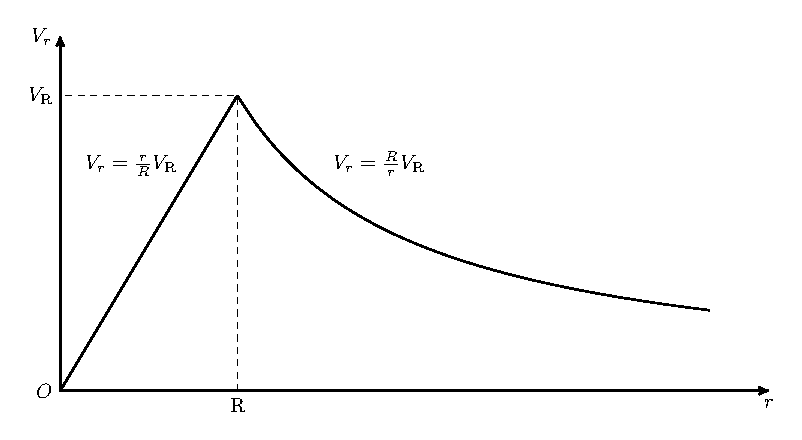
\includegraphics[width=0.6\textwidth]{Rankine.pdf}
	\caption{Rankine涡模型中切向速度沿涡半径的变化曲线图}
	\label{fig:Rankine}
\end{figure}


\section{缩尺龙卷风的CFD模拟}
本文选择Ward型龙卷风发生装置(Ward-type Tornado Vortex Chamber,下文简称Ward-TVC)\cite{ward1972exploration}的改进版(Purdue-TVC)\cite{church1979characteristics}进行数值模拟,Purdue-TVC的示意图见图\ref{fig:Ward-TVC}。
Davies-Jones\cite{davies1976laboratory}详细评述了各种龙卷风发生装置,认为Ward-TVC与实际发生的龙卷风之间具有较好的几何和动力学相似性(geometric and dynamic similarity)。

控制龙卷风风场的主要无量纲参数为\cite{lewellen1993tornado}:
高宽比$A$、涡流比$S$、雷诺数(Reynolds number)$\mathrm{Re}$、弗劳德数(Froude number)$\mathrm{Fr}=\left( \Delta P/ 2g\Delta \rho z\right)^{1/2}$;$\Delta P$为气压降、$\Delta \rho$为流域内空气密度的变化、$g$为重力加速度、$z$为距离地面的高度。
高宽比和涡流比的定义如下:
\begin{equation}
	A = H_0/R_0
\end{equation}
\begin{equation}
	S = V_t/2A V_r
\end{equation}
其中$R_0$为上升气流孔的半径,$H_0$为气流入口的高度(见图\ref{fig:Ward-TVC}),
$V_t$和$V_r$为$R_0$处的切向和径向入流速度。
试验\cite{ward1972exploration}\cite{church1979characteristics}\cite{snow1982review}和数值模拟\cite{davies1976laboratory}等说明涡流比是控制龙卷风风场特征的最主要参数。
图\ref{fig:swirl}展示了龙卷风风场结构随涡流比的增大而发生变化\cite{hangan2008swirl}。
\begin{figure}[!htbp]
	\centering
	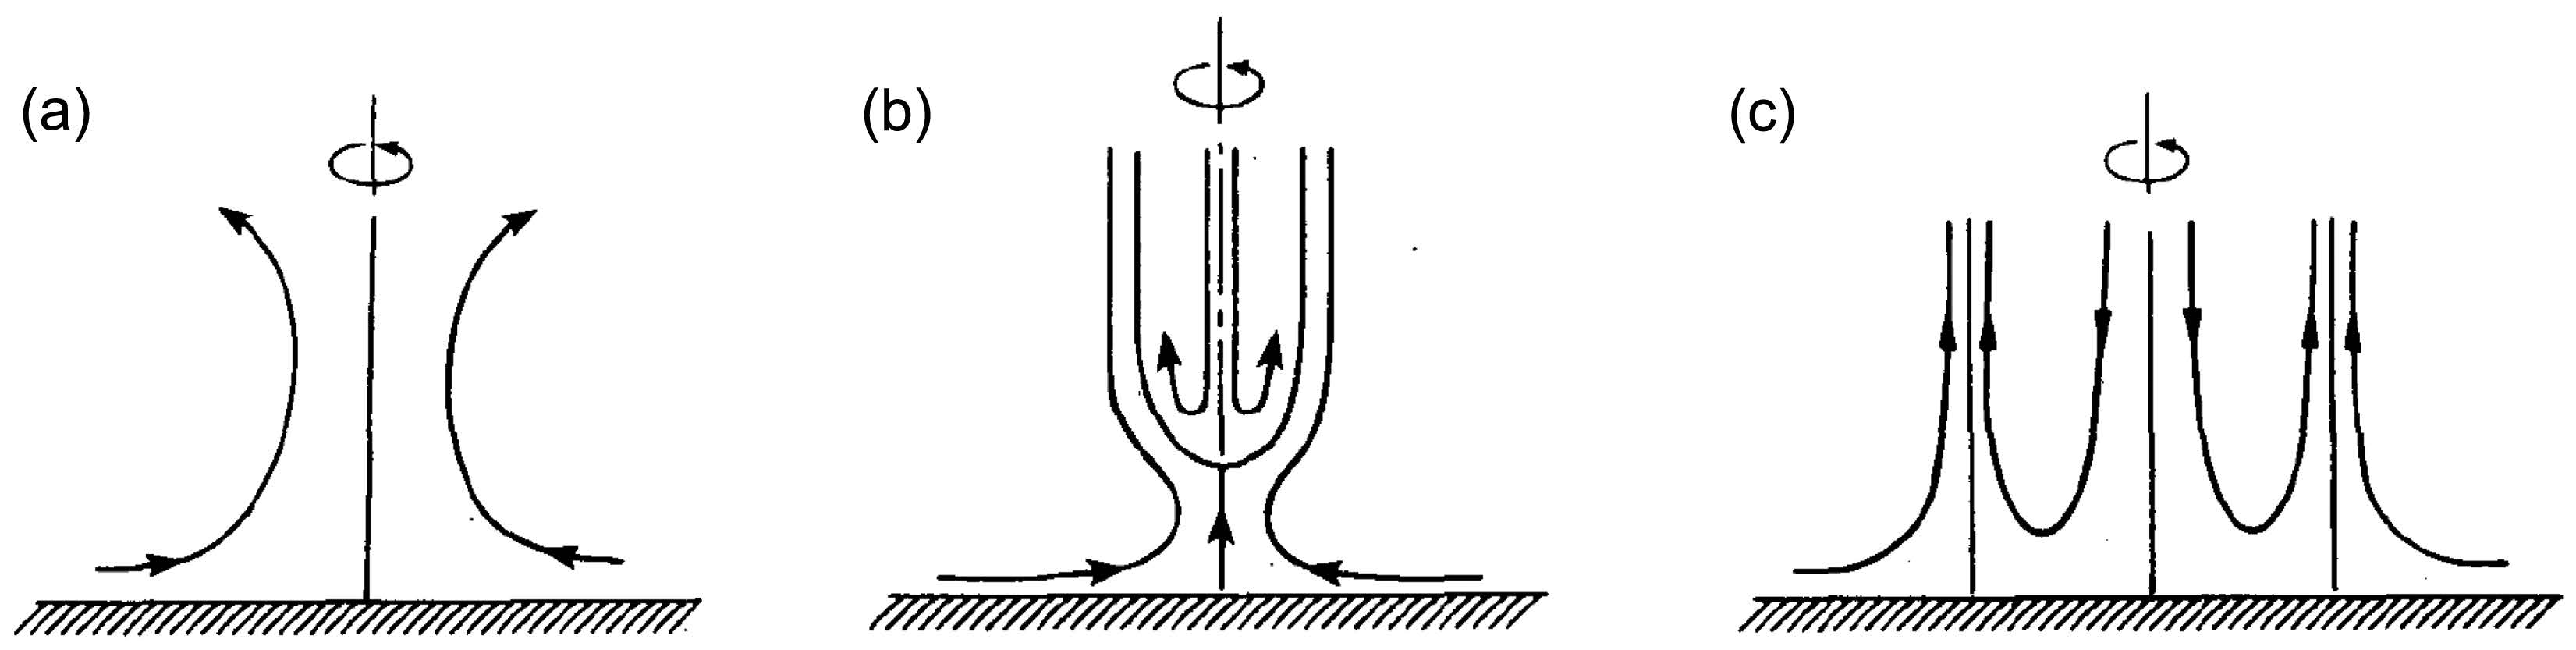
\includegraphics[width=\textwidth]{swirl_ratio_tornado_flow_pattern.jpg}
	\caption{增大涡流比引起龙卷风风场结构发生变化的示意图}\label{fig:swirl}
\end{figure}

随着涡流比的增大,龙卷风从射流状流场变化为单涡状涡旋(图\ref{fig:swirl}(a)),接着风场产生一个驻点、涡旋脱离地面(图\ref{fig:swirl}(b)),最后涡旋着地,分裂形成双涡状龙卷风(图\ref{fig:swirl}(c))。

本节主要介绍计算流体力学软件ANSYS Fluent模拟Ward-TVC的方法,并探讨涡流比对数值风场的影响。

\subsection{风场几何区域}
数值模拟的计算流域取Purdue-TVC的阴影区域,见图\ref{fig:Ward-TVC}。
为了与Baker\cite{baker1981boundary}的试验进行对比以验证数值风场的正确性,
取计算流域的尺寸及边界条件如图\ref{fig:tornado-domain}所示。
其中$X$轴对应龙卷风风场的径向,$Z$轴对应龙卷风风场的竖向。
\begin{figure}[!htbp]
	\begin{subfigure}[b]{0.5\textwidth}
		\centering
		\input{figures/tornado/Ward_TVC_sketch.pdf_tex}
		\caption{Purdue-TVC龙卷风发生装置示意图}\label{fig:Ward-TVC}
	\end{subfigure}
	\begin{subfigure}[b]{0.5\textwidth}
		\centering
		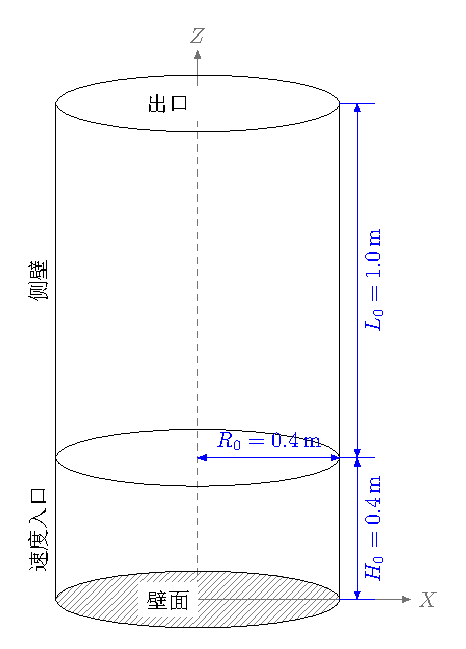
\includegraphics{domain.pdf}
		\caption{龙卷风数值模型的计算流域}\label{fig:tornado-domain}
	\end{subfigure}
	\caption{龙卷风发生装置和计算流域示意图}\label{fig:TVC-domain}
\end{figure}


\subsection{网格划分}
采用适应性良好的六面体结构化网格进行计算流域的划分。
初始网格数量大概为$300,000$,然后根据速度梯度和Y+进行自适应网格划分\cite{fluent2015user}。由于工程实际主要关注近地面附近龙卷风对结构的作用,
故细分主要针对近地面流域处的网格。不断加密网格直到近地面最大切向速度和最大切向速度所在半径的位置前后两次计算结果相差小于$5\%$。最后根据计算机的能力及计算结果的有效性,采用的网格数量为$1,536,000$。


\subsection{湍流模型}
龙卷风风场是旋流流场,根据Launder\cite{launder1989second}的研究,采用雷诺应力方程模型 (RSM)较为合适。
模型参数为:$C_{\mu}=0.09$; $C_{1\varepsilon}=1.44$; $C_{2\varepsilon}=1.92$; 
$C1-ps=1.8$; $C2-ps=0.6$; $C1'-ps=0.5$; $C2'-ps=0.3$。
湍流动能(TKE)普朗特数为 $1$; 湍动耗散率(TDR)普朗特数为 $1.3$。

\subsection{边界条件}
速度入口处径向和切向速度分布采用如下形式:
\begin{equation}\label{eqn:Vr}
	V_r(z) = V_0 \times (z/z_0)^{1/7}
\end{equation}
\begin{equation}\label{eqn:Vt}
	V_t(z) = 2 \times S \times V_r(z)
\end{equation}
式中,$V_r$为径向速度,$V_t$为切向速度,$V_0$为参考速度,$z_0$为参考高度,$S$为涡流比。

图\ref{fig:bc-inlet}为公式\eqref{eqn:Vr}和\eqref{eqn:Vt}所定义的风速分布与Baker\cite{baker1981boundary}试验的对比。
注意到试验风速分布与试验装置有关,而非实际的大气边界层风速分布。
公式\eqref{eqn:Vr}和\eqref{eqn:Vt}类似于大气边界层风速分布,并尽可能与Baker\cite{baker1981boundary}试验保持一致。
\begin{figure}[!htbp]
	\centering
	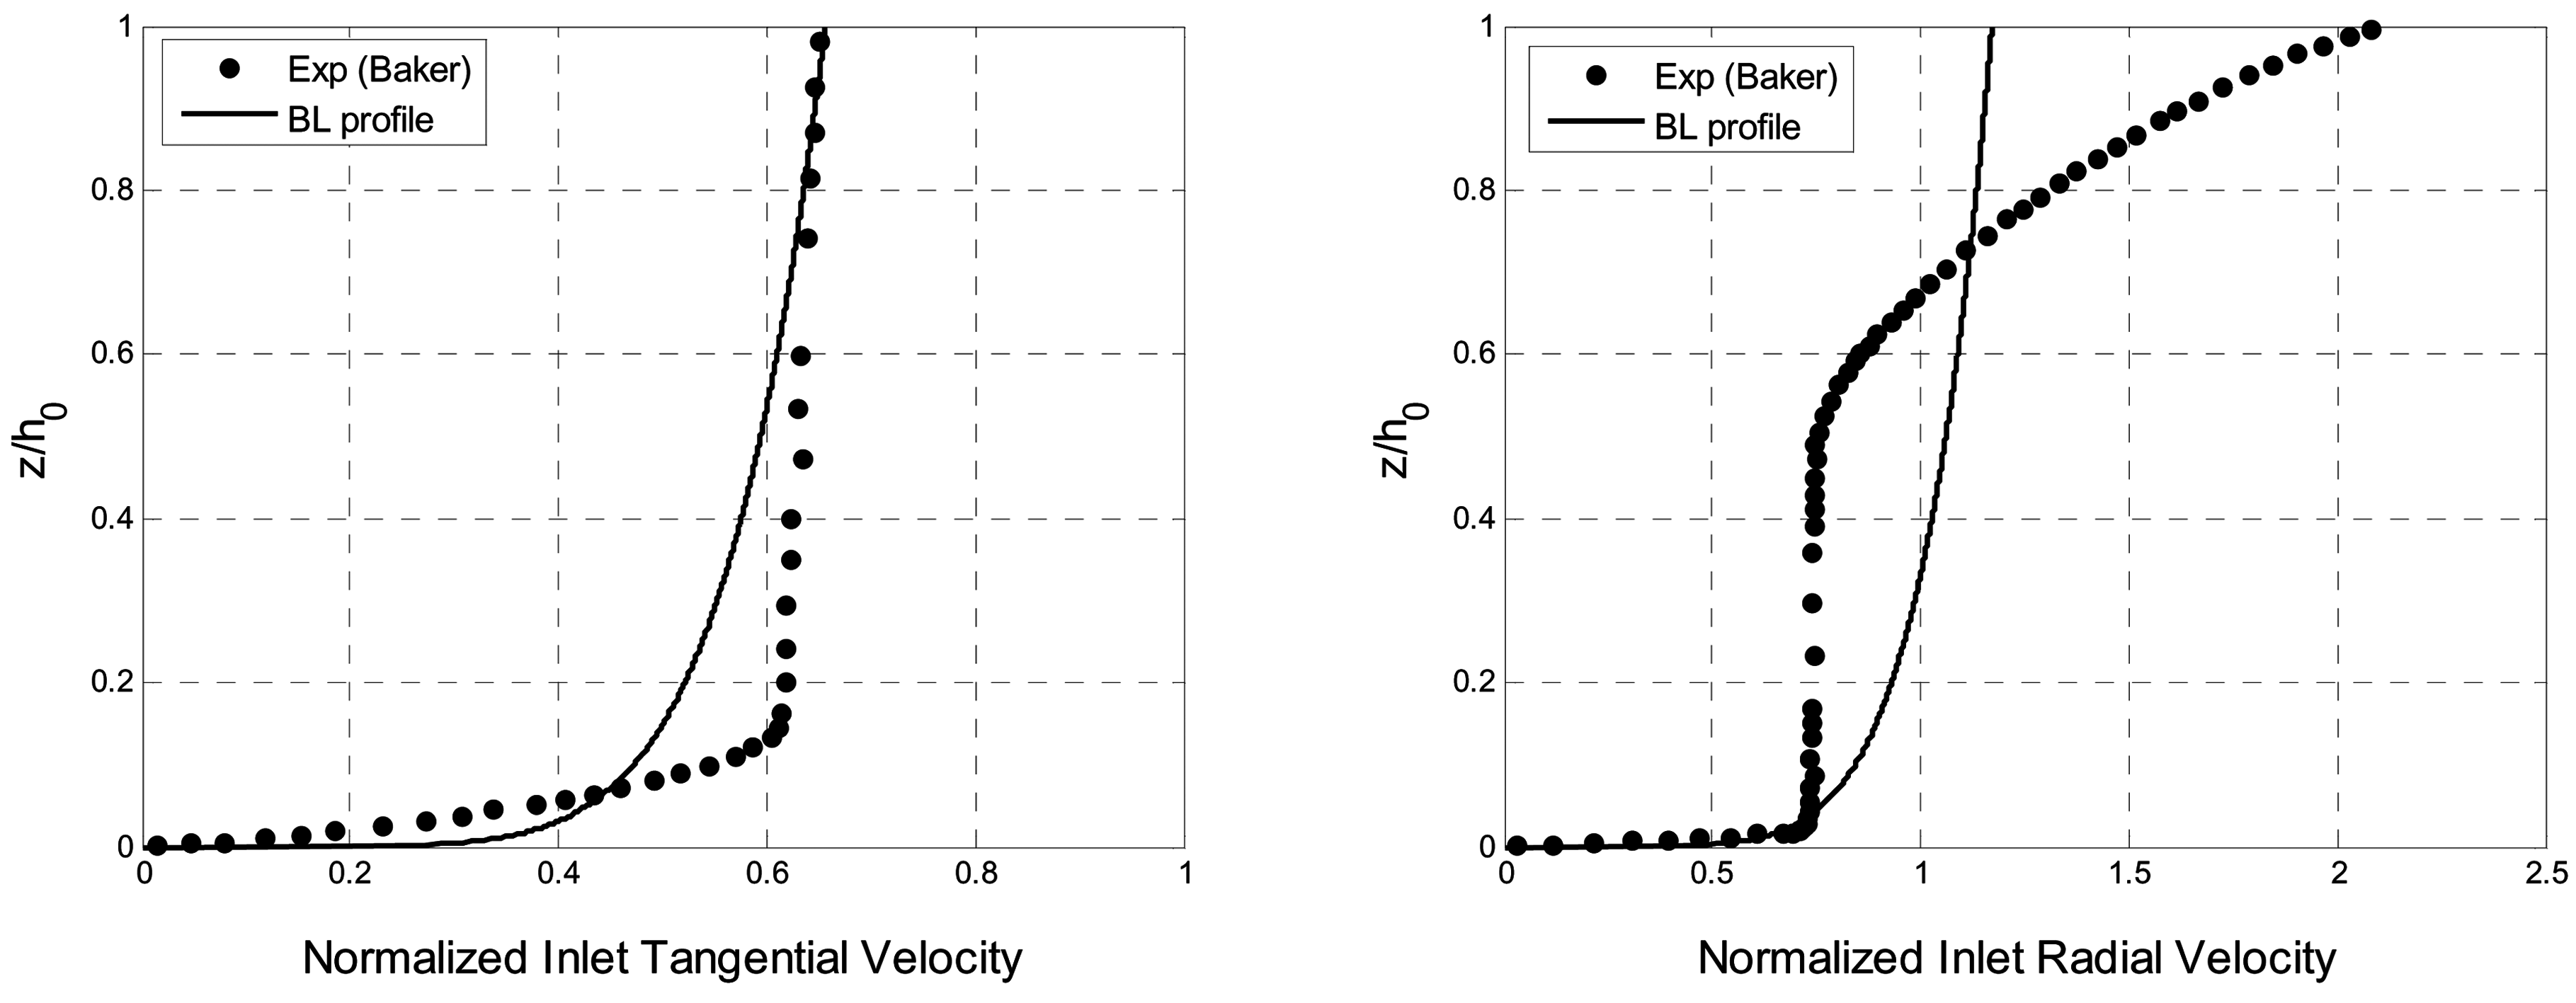
\includegraphics[width=\textwidth]{bc_inlet.png}
	\caption{入口处规格化切向和径向速度与Baker\cite{baker1981boundary}试验的对比}
	\label{fig:bc-inlet}
\end{figure}

试验表明,沿壁面法线方向的不同距离,可以将近壁面区域分成三层区域。
最里层,又称粘性底层,流动区域很薄,粘性力在动量、热量及质量交换中都起主导作用;
最外层为对数率层,粘性力不起主要作用;
两层之间的区域为过渡层,粘性力作用与湍流作用相当。

为描述粘性底层和对数率层内的流动,现引入无量纲参数$u^{+}$和$y^{+}$:
\begin{equation}
	u^{+} = \frac{u}{u_{\tau}}
\end{equation}
\begin{equation}
	y^{+} = \frac{y u_{\tau}}{\nu} = \frac{y}{\nu} \sqrt{\frac{\tau_w}{\rho}}
\end{equation}
式中:$u$是流体的时均速度、$u_{\tau}=\sqrt{\tau_w/\rho}$为壁面摩擦速度、$\tau_w$为壁面处切应力、$\nu$为空气动粘度系数、$y$为壁面第一层节点到壁面的距离。

以$y^{+}$的对数为横坐标,以$u^{+}$为纵坐标,可将壁面区域内的三个区域表示为图\ref{fig:uplus}所示\cite{fluent2015theory}。
\begin{figure}[!htbp]
	\centering
	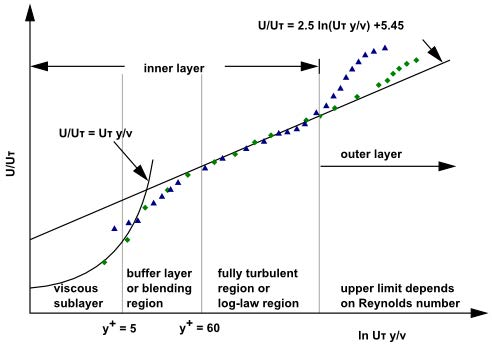
\includegraphics[width=0.6\textwidth]{figures/tornado/uplus.jpg}
	\caption{近壁面区域划分}\label{fig:uplus}
\end{figure}

通常有两种方法模拟近壁面区域:
一种采用“壁面方程”的半经验公式模拟受粘性力影响较大的区域,能够较好地修正湍流模型,解决壁面的存在对流场的影响;
另一种方法采用低$\mathrm{Re}$数的$k-\varepsilon$模型来求解粘性底层和过渡层,越靠近壁面,网格划分就越细,这种方法被称为“近壁面模型”法。
图\ref{fig:wall-treatment}为两种方法的对比\cite{fluent2015theory}。
\begin{figure}[!htbp]
	\centering
	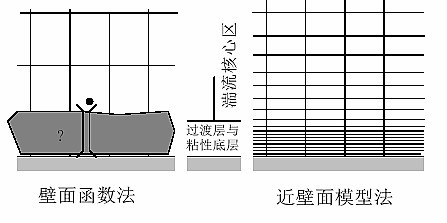
\includegraphics[width=0.8\textwidth]{wall_treatment.jpg}
	\caption{近壁面区域处理方法}
	\label{fig:wall-treatment}
\end{figure}

本文地面处采用强化壁面函数(Enhanced wall treatment\cite{fluent2015user}),需要对近壁面的网格进行细化。
边界层网格节点是否合适需要检查计算后的$y^{+}$值。
$y^{+}=u_{\tau} y/\nu$小于$1.5$能取得较好效果。

Smith的数值模拟\cite{smith1987effect}说明了侧壁的边界条件的选取对汇集区风场(主要关注的区域)的影响很小。
因此选择无滑壁面条件。

Purdue-TVC出口处设置了蜂窝板,能使气流竖直流出,还能阻止排风机对涡旋的影响。
试验中排风机驱动了流场运动,而在数值模型中,入口风速驱动了流场运动,且不包含排风机的影响,因此数值模型出口处不需设置代表直流蜂窝板的边界条件。根据Smith\cite{smith1987effect}的论述,上边界更合适的边界条件为压强出口边界条件(pressure-outflow)。
此边界条件假设除压强外的所有物理量在边界的法向梯度为零\cite{fluent2015user}。

\subsection{控制方程及求解选项}
控制方程采用非定常雷诺平均纳维-斯托克斯方程(Unsteady Reynolds Averaged Navier-Stokes, RANS)。
时间离散采用一阶隐性格式,压强速度场的耦合采用压力修正的分离式算法,SIMPLEC算法。
动量、TKE、TDR和雷诺应力采用二阶迎风格式。



\section{龙卷风数值模拟结果及其正确性验证}\label{sec:tornado}
图\ref{fig:tornado-domain}所示的风场几何区域,建立柱面坐标系$\{O:r \theta z\}$。
本文主要关注在柱面坐标系下数值风场的速度特征,其中径向(radial)、切向(tangential)、竖向(axial)风速分别记为$V_r(r,\theta,z)$、$V_t(r,\theta,z)$和$V_a(r,\theta,z)$。

考虑到龙卷风风场具有轴对称性,故对数值风场速度分布沿圆周($r=$常数)进行平均,消除速度随$\theta$的变化,得到轴对称的风场$V_r(r,z)$、$V_t(r,z)$和$V_a(r,z)$。

% 将上述轴对称风场与Baker试验\cite{baker1981boundary}结果及多普勒雷达实测风场进行对比,以验证数值风场的正确性。
% 并探讨缩尺龙卷风数值风场转化为足尺风场的方法。

\subsection{Baker试验对比}
Baker利用Purdue-TVC进行了龙卷风风场的试验模拟\cite{baker1981boundary},选取$S=0.28$的风场在$r/R_0=0.1025$和$r/R_0=0.2125$处风速各分量随高度变化曲线与数值风场进行对比。
将高度以$R_0$进行无量纲化,速度以入口平均径向速度$U_0=Q/(R_0 H_0)$进行无量纲化,其中$2\pi Q$为速度入口边界处的流量。
将\eqref{eqn:Vr}定义的速度入口边界的径向速度代入可得:
\begin{equation}
	U_0 = \frac{Q}{R_0 H_0} = \frac{R_0 \int_0^{H_0} V_r(z)\,\mathrm{d}z}{R_0 H_0} = \frac{\int_0^{H_0} V_0 (z/z_0)^{1/7}\,\mathrm{d}z}{H_0} = \frac{7}{8} V_0 \left(\frac{H_0}{z_0}\right)^{1/7}
\end{equation}

图\ref{fig:cfd_vs_exp_Vr}、图\ref{fig:cfd_vs_exp_Vt}和图\ref{fig:cfd_vs_exp_Va}分别为数值风场(CFD)与Baker试验无量纲化径向、切向和轴向风速随高度变化的对比图。
二者总体上吻合较好。

\begin{figure}[!htbp]
	\centering
	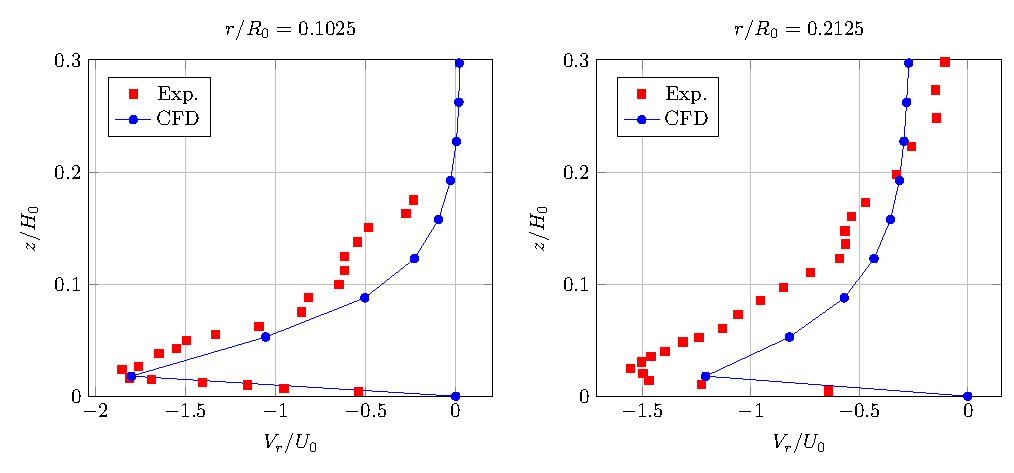
\includegraphics[width=1.0\textwidth]{cfd_vs_exp_Vr.pdf}
	\caption{数值风场与Baker试验无量纲化径向速度随高度变化的对比,$S=0.28$}
	\label{fig:cfd_vs_exp_Vr}
\end{figure}
\begin{figure}[!htbp]
	\centering
	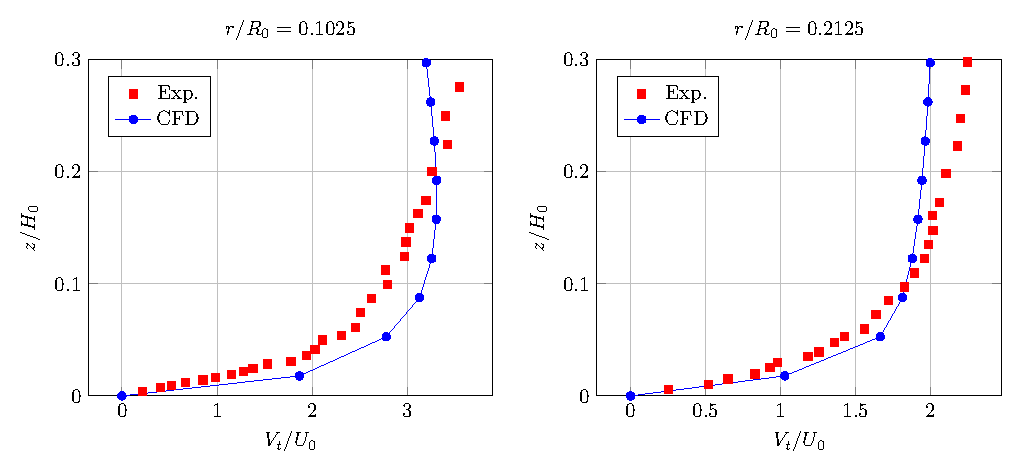
\includegraphics[width=1.0\textwidth]{cfd_vs_exp_Vt.pdf}
	\caption{数值风场与Baker试验无量纲化切向速度随高度变化的对比,$S=0.28$}
	\label{fig:cfd_vs_exp_Vt}
\end{figure}
\begin{figure}[!htbp]
	\centering
	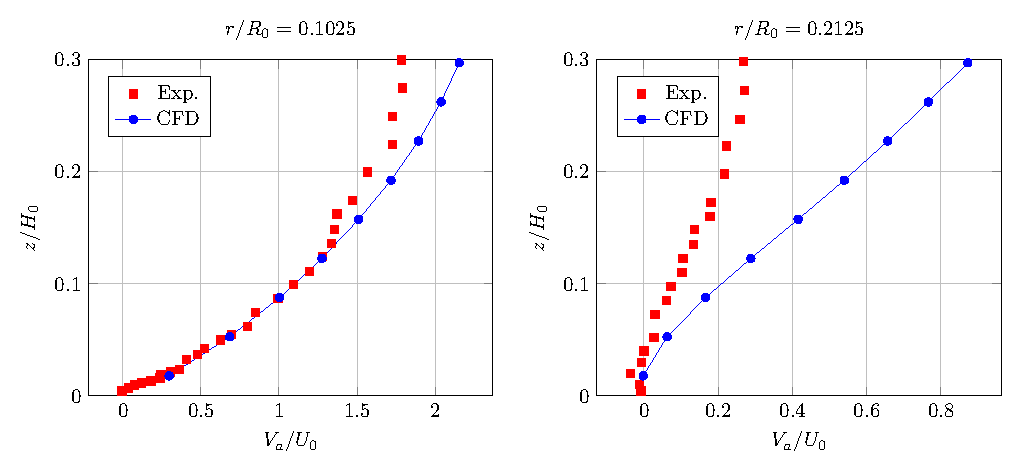
\includegraphics[width=1.0\textwidth]{cfd_vs_exp_Va.pdf}
	\caption{数值风场与Baker试验无量纲化竖向速度随高度变化的对比,$S=0.28$}
	\label{fig:cfd_vs_exp_Va}
\end{figure}

\subsection{数值风场的风速分布特征}
图\ref{fig:Vt-x=0}为计算流域轴向剖面($X=0$)处切向速度云图。
从图中可以明显看出涡旋中心处切向速度接近于零;
图\ref{fig:Vt-z=30mm}为\SI{30}{mm}高度处的切向速度云图,可以看出流域的涡旋接近中心轴线,并能显示出漏斗状形态,显示了龙卷风风场具有很好的涡旋特性。
由图\ref{fig:Vt}可知龙卷风涡旋中心的切向速度较小,在核心半径处达到最大,而后随着远离涡旋中心的距离增大而逐渐减小。
且在核心半径内,切向速度的变化较快,而远离核心半径时,变化逐渐缓和,与Rankine模型吻合较好。
此外还可看出随着离地高度的增加,核心半径有所增大,而最大切向风速呈逐渐减小的趋势。
\begin{figure}[!htbp]
	\begin{subfigure}[b]{0.5\textwidth}
		\centering
		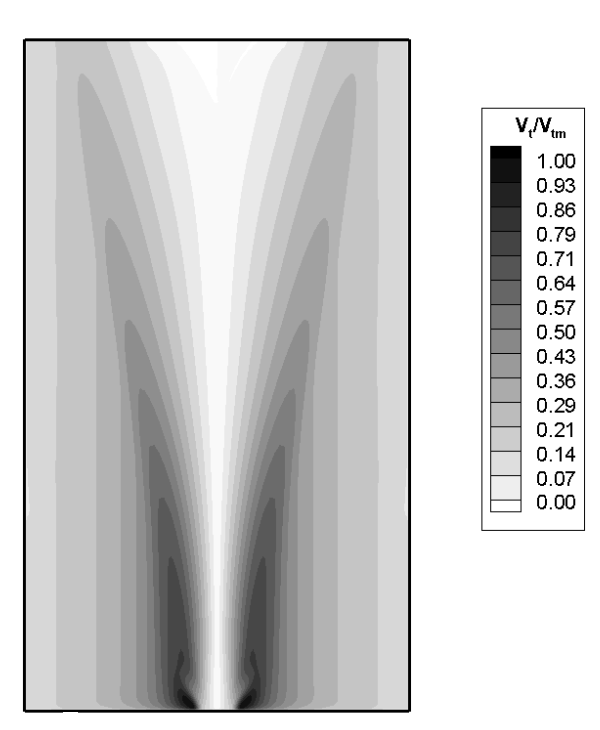
\includegraphics[width=\textwidth]{Vt_x=0.png}
		\caption{轴向剖面($X=0$)}\label{fig:Vt-x=0}
	\end{subfigure}
	\begin{subfigure}[b]{0.5\textwidth}
		\centering
		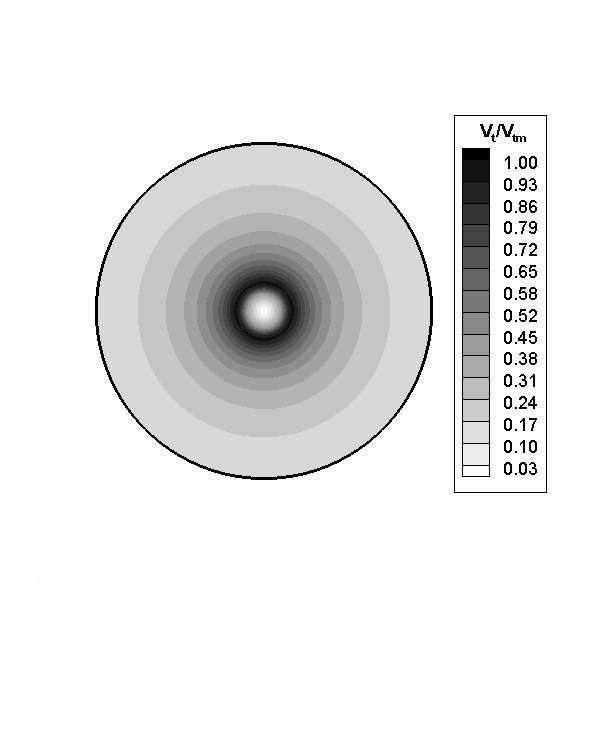
\includegraphics[width=\textwidth]{Vt_z=30mm.png}
		\caption{水平剖面($Z=\SI{30}{mm}$)}\label{fig:Vt-z=30mm}
	\end{subfigure}
	\caption{切向速度云图}\label{fig:Vt-contour}
\end{figure}

\begin{figure}
	\centering
	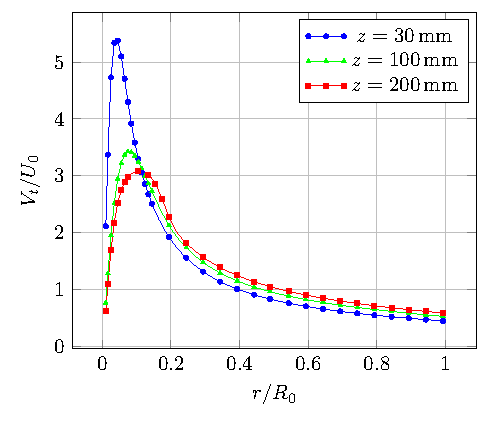
\includegraphics[width=0.6\textwidth]{Vt.pdf}
	\caption{数值风场不同高度处切向速度沿径向的变化图,$S=0.28$}
	\label{fig:Vt}
\end{figure}

\subsection{数值风场的风压分布特征}
图\ref{fig:P-x=0}和图\ref{fig:P-z=30mm}分别给出了计算流域轴向剖面($X=0$)和水平剖面($Z=\SI{30}{mm}$)处风压云图,$P_m$是风场最大静压,为负压。
可以看出龙卷风中心处离地面一定高度范围内存在很强的负压,且随着半径的增加而逐渐减小。

图\ref{fig:p}给出了三种不同高度处的风压沿径向的分布,可以看出不同高度处风压分布接近一致。

\begin{figure}[!htbp]
	\begin{subfigure}[b]{0.5\textwidth}
		\centering
		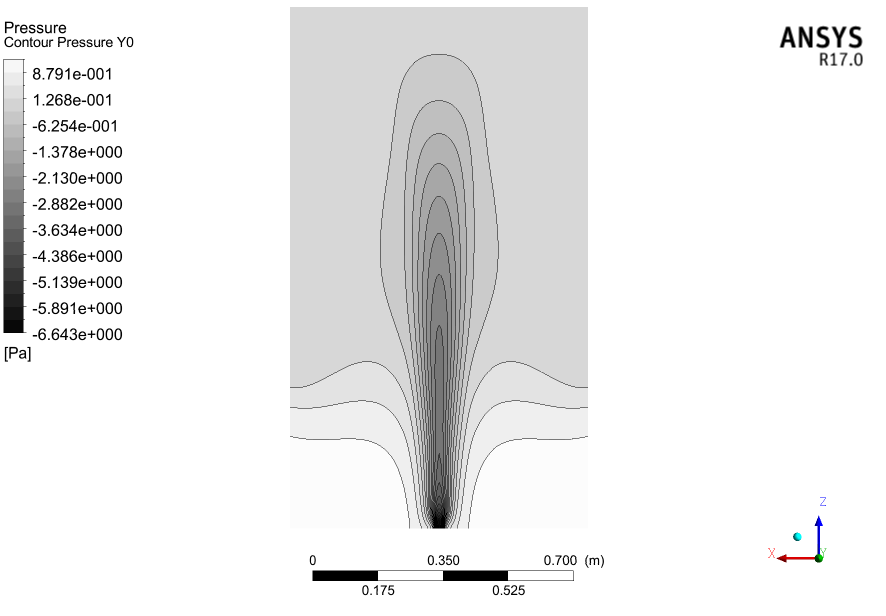
\includegraphics[width=\textwidth]{P_x=0.png}
		\caption{轴向剖面($X=0$)}\label{fig:P-x=0}
	\end{subfigure}
	\begin{subfigure}[b]{0.5\textwidth}
		\centering
		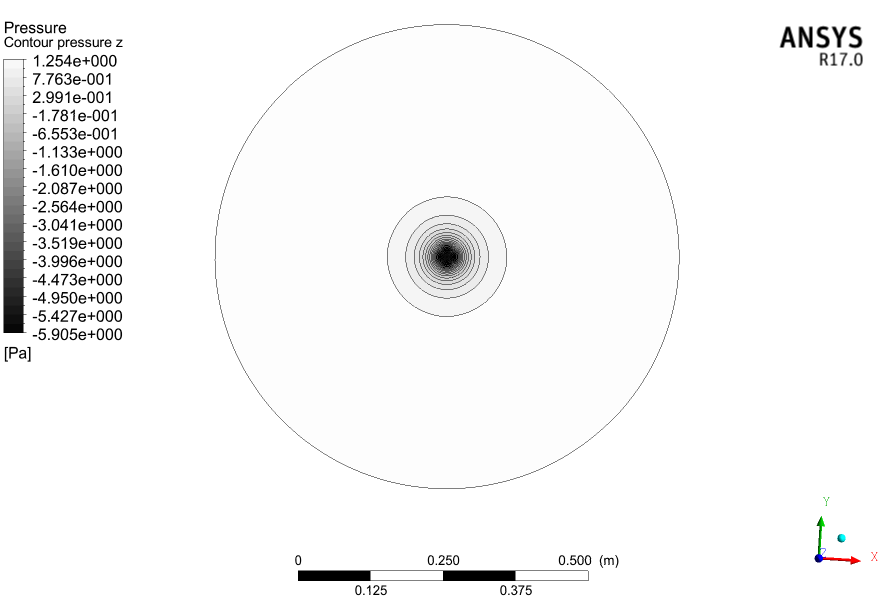
\includegraphics[width=\textwidth]{P_z=30mm.png}
		\caption{水平剖面($Z=\SI{30}{mm}$)}\label{fig:P-z=30mm}
	\end{subfigure}
	\caption{风压云图}\label{fig:p-contour}
\end{figure}

\begin{figure}[!htbp]
	\centering
	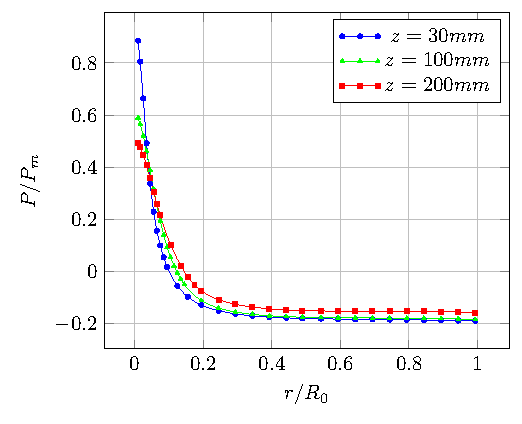
\includegraphics[width=0.6\textwidth]{p.pdf}
	\caption{数值风场不同高度处风压沿径向的变化图}
	\label{fig:p}
\end{figure}

\section{足尺龙卷风CFD模拟}

\subsection{长度相似比和速度相似比}

足尺风场选用1998年5月发生在美国南达科他州Spencer地区的实测龙卷风风场,
这些数据由车载式多普勒雷达采集,Wurman等人有详细的介绍\cite{wurman2002multiple}\cite{alexander2005spencer}\cite{wurman2005spencer}。

采集的风场在不同竖向高度处、\SI{2}{km}$\times$\SI{2}{km}的水平区域内(水平测点间距为\SI{20}{m})。
将原始风场去除龙卷风平移速度,得到涡旋风场,并利用最小二乘原理将速度场沿圆周平均,以消除多涡等因素的影响。
最终得到的龙卷风切向速度随离开涡旋中心径向距离的变化关系如图\ref{fig:Vt-full}所示。
\begin{figure}[!htbp]
	\centering
	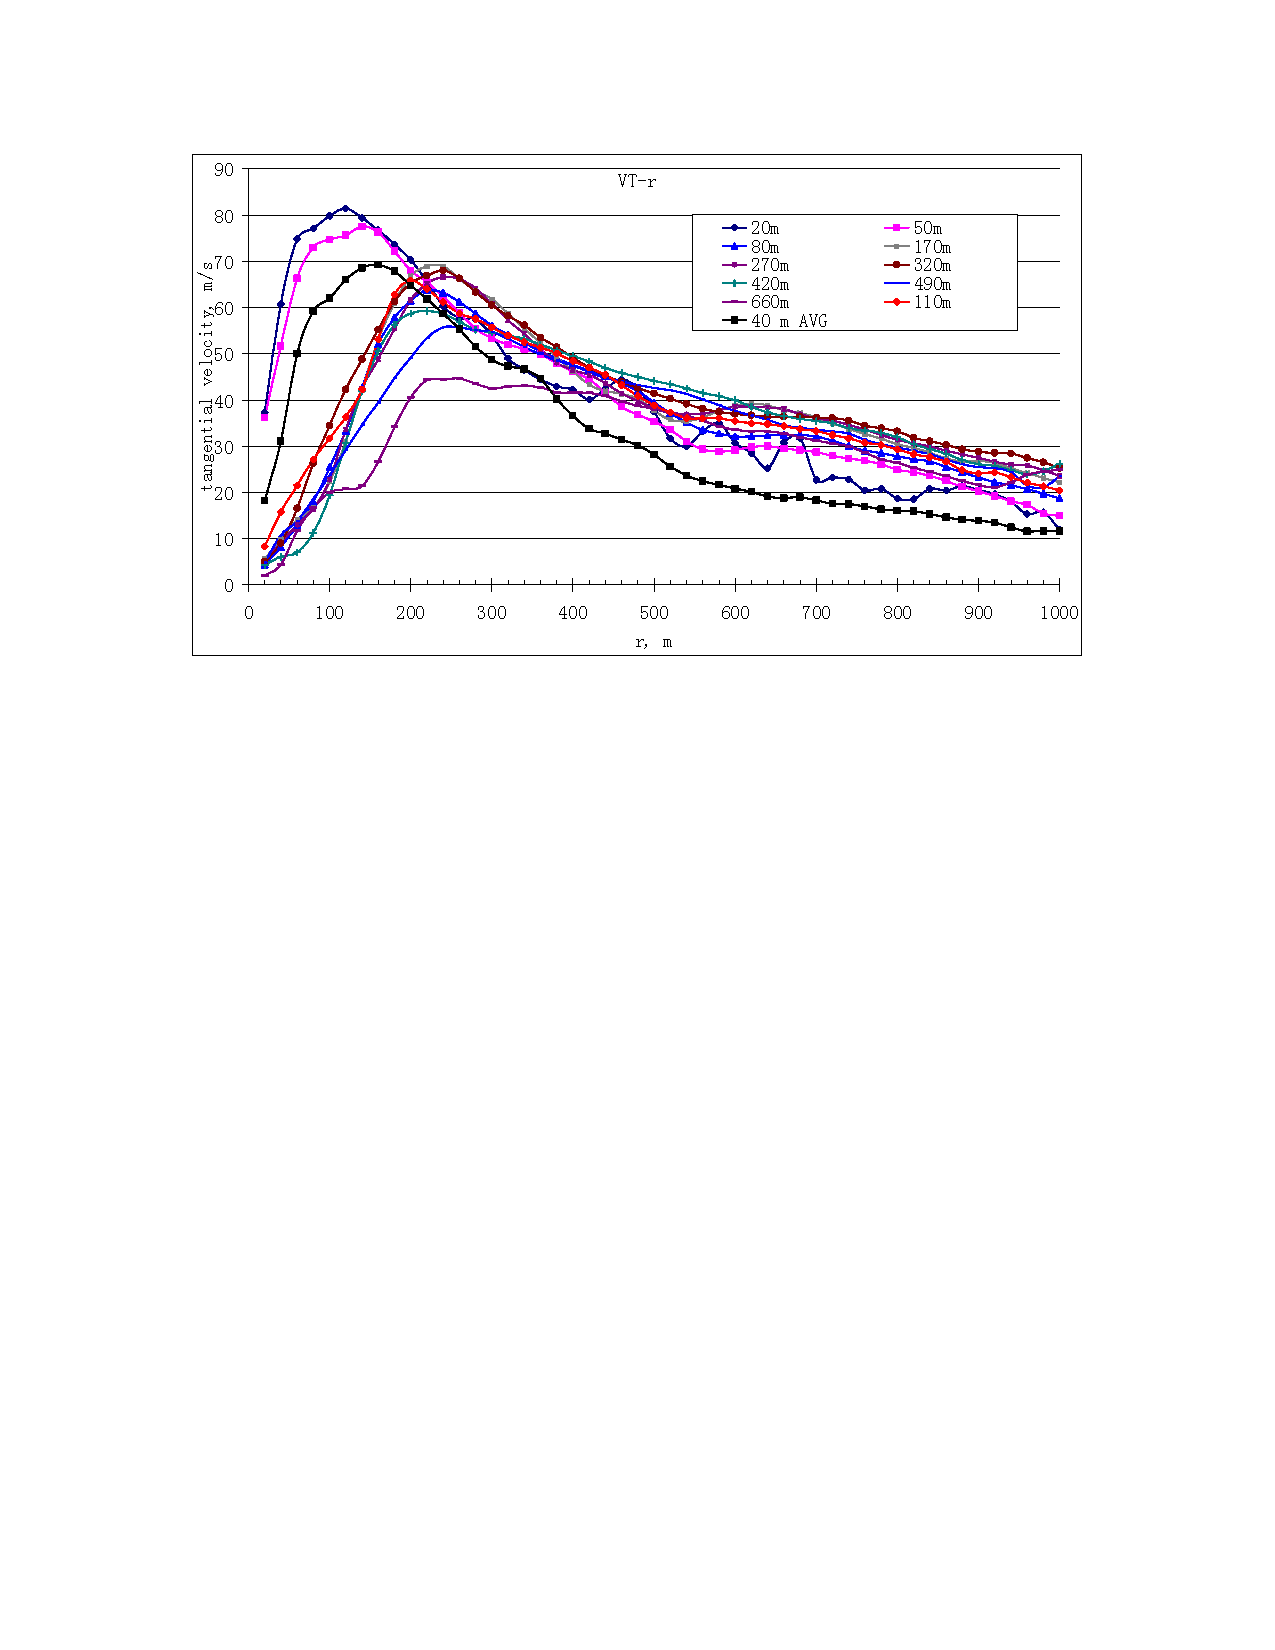
\includegraphics[width=0.8\textwidth]{Vt_full.pdf}
	\caption{实测风场在不同高度处切向速度与径向距离的关系曲线\cite{sarkar2005velocity}}
	\label{fig:Vt-full}
\end{figure}

考虑缩尺风场和实测风场的最大切向速度及其发生位置$V_t(r_{c\,\mathrm{max}}, z_{\mathrm{max}})$,
其中$r_{c,\mathrm{max}}$为风场在$z_{\mathrm{max}}$高度处的核心半径(龙卷风最大切向速度点距龙卷风中心的距离)。
速度相似比和长度相似比定义为\cite{hangan2008swirl}:
\begin{equation}
	V_s  =  \frac{V_{t,\mathrm{max}}^{\text{Full}}}{V_{t,\mathrm{max}}^{\text{CFD}}}
\end{equation}
\begin{equation}
	L_s  =  \frac{r_{c,\mathrm{max}}^{\text{Full}}}{r_{c,\mathrm{max}}^{\text{CFD}}} \quad \text{or} \quad \frac{z_{c,\mathrm{max}}^{\text{Full}}}{z_{c,\mathrm{max}}^{\text{CFD}}}
\end{equation}

本文模拟的缩尺龙卷风速度相似比为$V_s=60$。
文献\cite{hangan2008swirl}研究了长度相似比$L_s$随涡流比$S$变化的情况,见图\ref{fig:Ls-S}。
发现两种方式定义的长度相似比$L_s$随涡流比$S$的增大逐渐趋向于定值。
本文取长度相似比$L_s$为该定值$4000$。

\begin{figure}[!htbp]
	\centering
	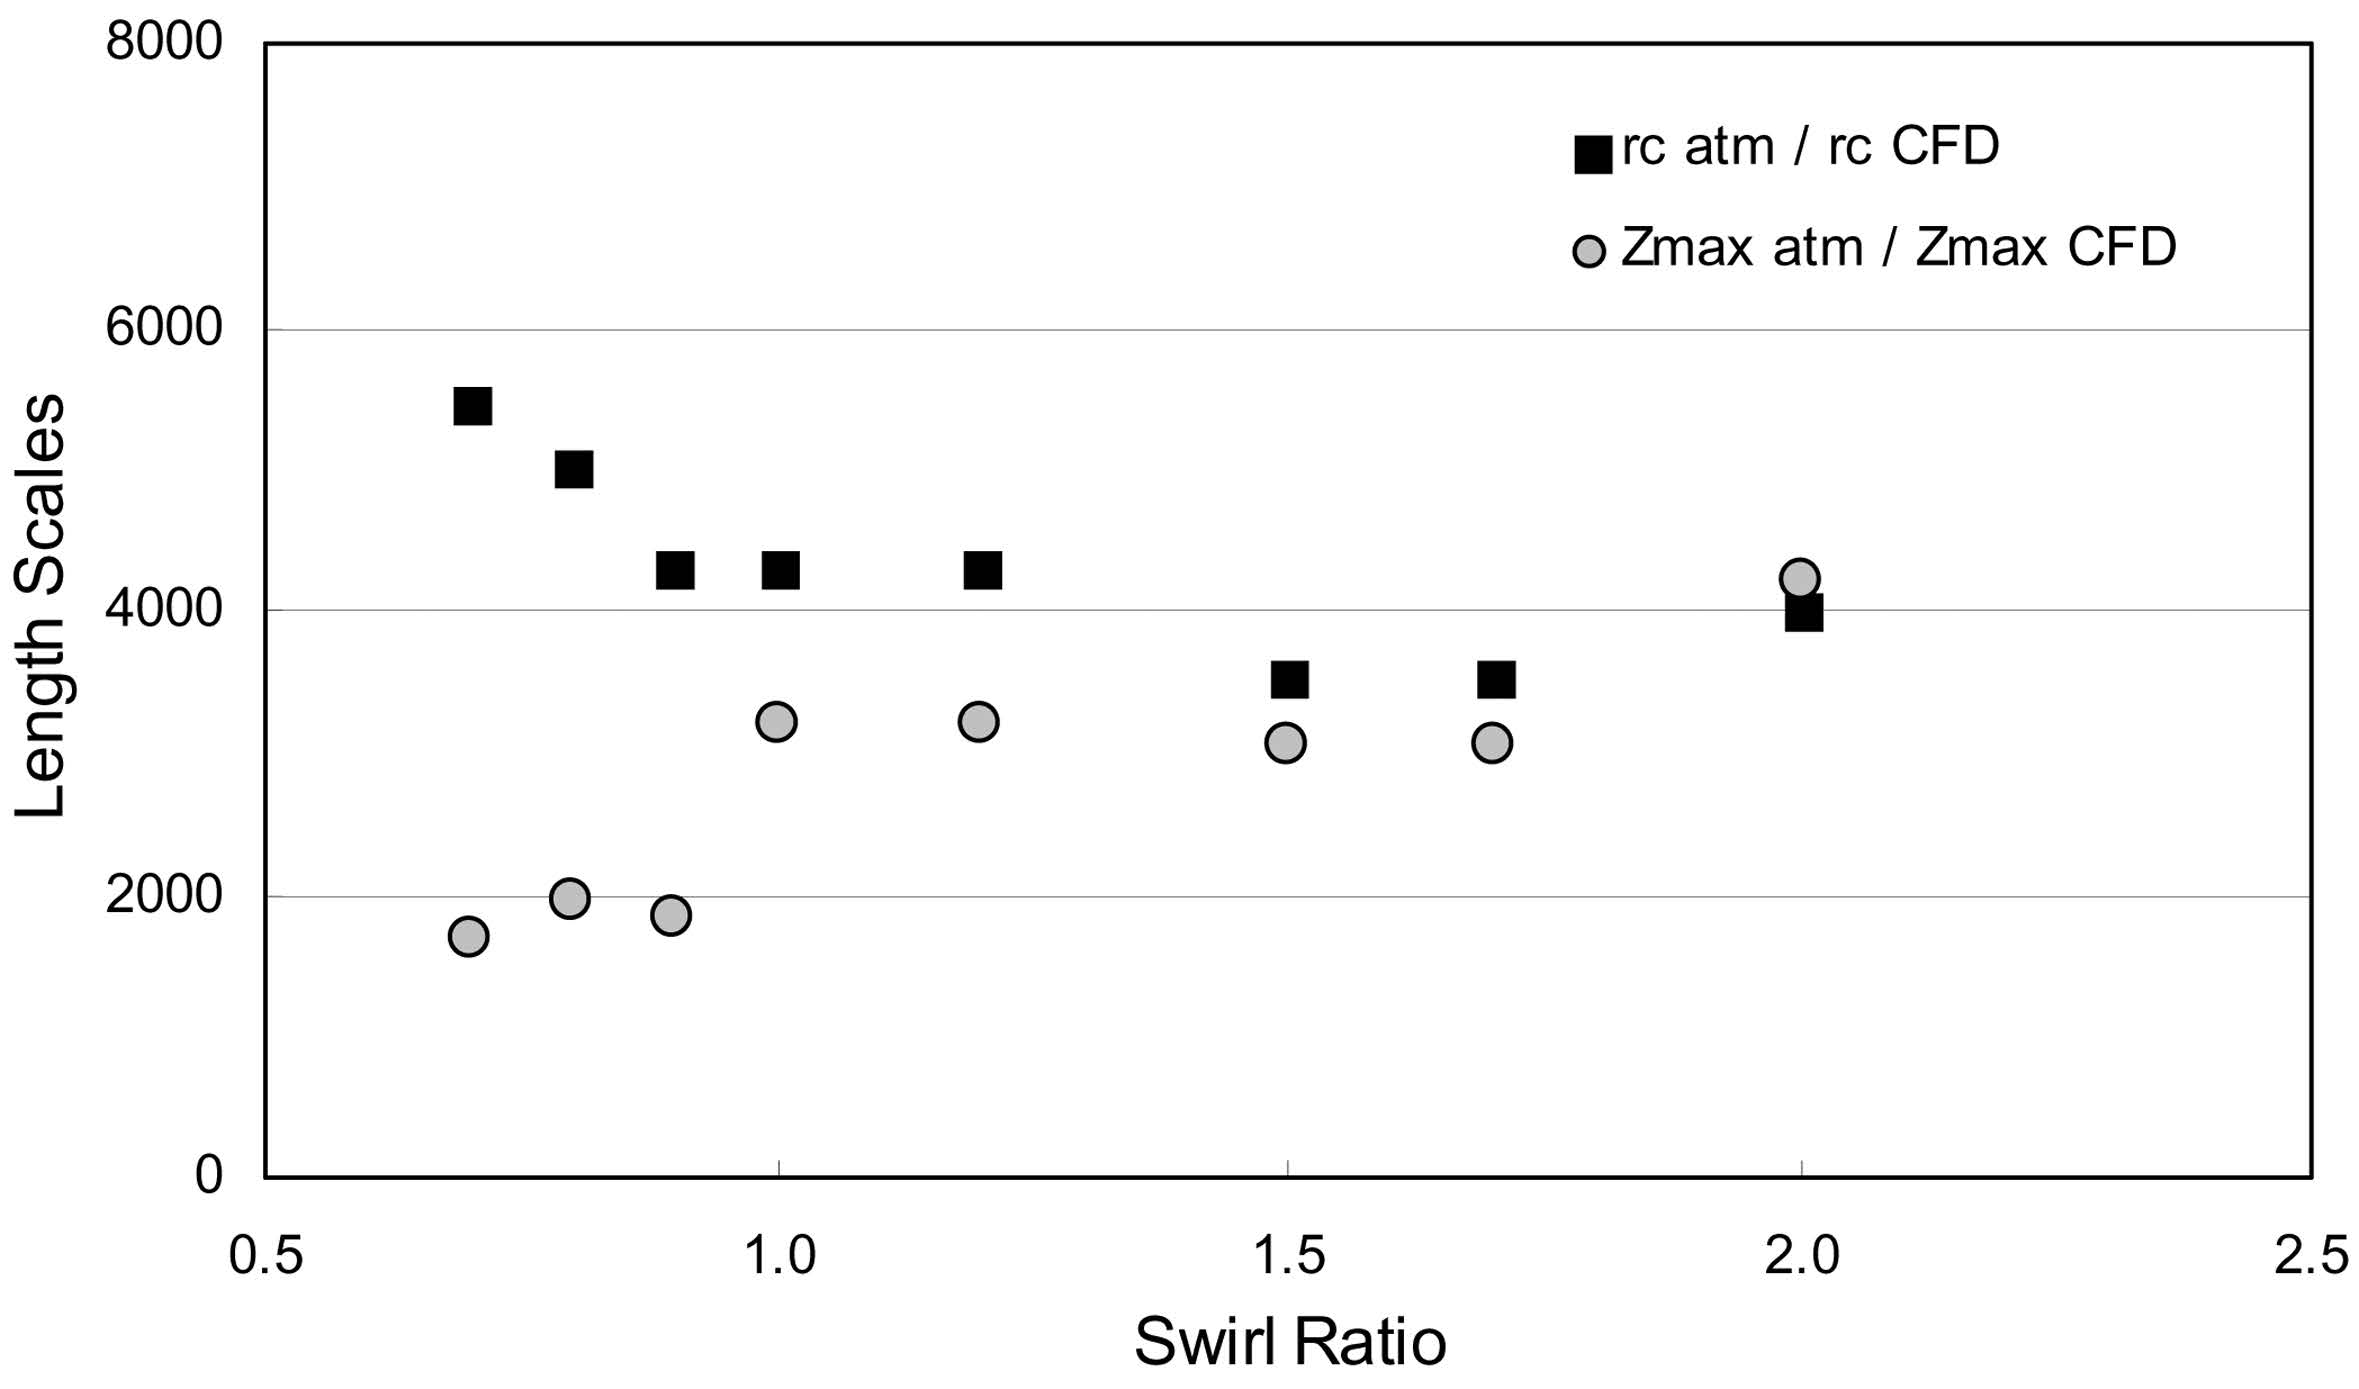
\includegraphics[width=0.8\textwidth]{ls_vs_s.jpg}
	\caption{长度相似比$L_s$随涡流比$S$的变化\cite{hangan2008swirl}}
	\label{fig:Ls-S}
\end{figure}

\subsection{足尺龙卷风风场CFD模拟}\label{sec:full-tornado}

本节利用长度相似比$L_s$和速度相似比$V_s$将缩尺CFD风场转化为足尺龙卷风风场。
首先,将缩尺风场的计算流域(见图\ref{fig:TVC-domain})的底面半径放大为$L_s\times R_0$、
速度入口高度放大为$L_s \times H_0$;
入口边界条件的径向和切向入流速度设置为:
\begin{equation}
	V_r^{\text{Full}}(z) = (V_s V_0)\times\left[z/(L_s z_0)\right]^{1/7}
\end{equation}
\begin{equation}
	V_t^{\text{Full}}(z) = 2 \times S \times V_r^{\text{Full}}(z)
\end{equation}

比较足尺龙卷风风场与Spencer龙卷风实测风场在不同高度处的切向速度沿径向的分布,
见图\ref{fig:cfd-Spencer}所示,二者整体上吻合较好。

\begin{figure}[!htbp]
	\centering
	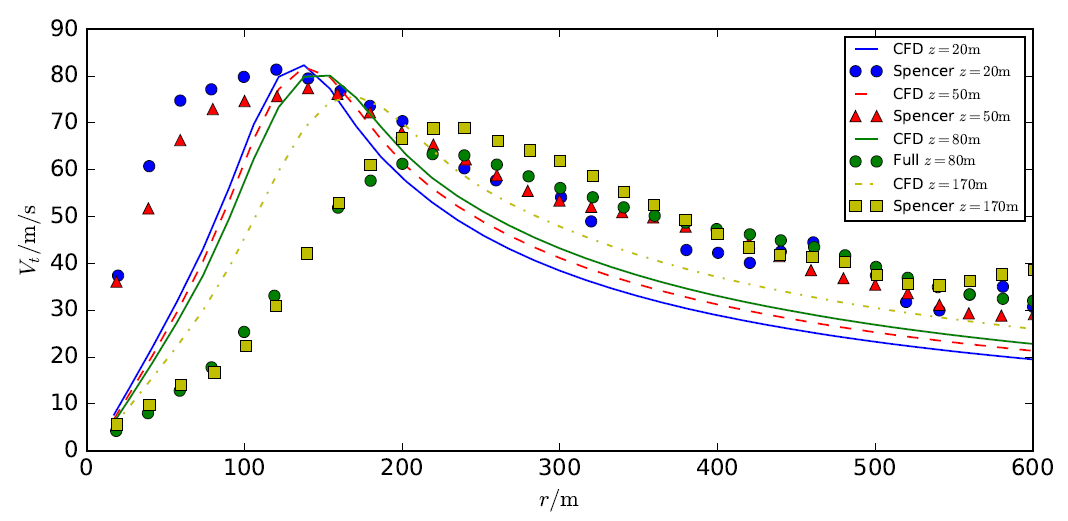
\includegraphics[width=0.8\textwidth]{cfd-vs-Spencer.png}
	\caption{CFD足尺风场与Spencer实测风场切向速度分布比较}
	\label{fig:cfd-Spencer}
\end{figure}
